% Copyright (c) 2022 Tobias Briones. All rights reserved.
% SPDX-License-Identifier: CC-BY-SA-4.0
%
% This source code is part of
% https://github.com/tobiasbriones/cp-unah-is911-microprocessors and is
% licensed under the Creative Commons Attribution Share Alike 4.0
% International License found in the LICENSE file in the root
% directory of this source tree or at https://spdx.org/licenses/CC-BY-SA-4.0

\documentclass[conference]{IEEEtran}
\usepackage{preamble}

\title{ESP32 CON C++ Y MICROPYTHON}
\author{
    
\includegraphics[width = 40mm]{images/logo-unah}\\[8ex]
    \IEEEauthorblockN{Tobias Briones}
    \IEEEauthorblockN{tobias.briones@unah.hn}
    \IEEEauthorblockA{\textit{Universidad Nacional Autónoma de Honduras} \\
    \textit{Ingeniería de Sistemas} \\
    \textit{I PAC 2022} \\
    \textit{IS911-MICROPROCESADORES}} \\\vspace*{20pt} \normalsize  \\
    \today
}

\begin{document}

    \maketitle

    \begin{abstract}
        En este marco teórico se investigan la información de entrada para
        empezar a emplear la tarjeta microcontrolador ESP32 así como ejemplos
        de código en C++ Arduino IDE y MicroPython.
    \end{abstract}

    \tableofcontents

    \import{}{footer}

    \section{Introducción}\label{sec:introduction}

    ESP32 es una tarjeta microcontrolador de bajo costo
    \cite{wikipedia-esp32-2022} similar a las demás tarjetas conocidas como
    Arduino y Raspberry Pi Pico. Esta puede ser programada mediante Arduino
    IDE al hacer la configuración correspondiente y además mediante
    MicroPython también. Cuenta con una gran cantidad de características
    similares a las de este tipo de tarjetas microcontrolador de entrada.

    \bigbreak

    La tarjeta ESP32 tiene una gran capacidad de conexión inalámbrica tanto
    WiFi como Bluetooth, posee grandes integraciones en su diseño, bajo
    consumo de potencia y un diseño robusto
    \cite{espressif-systems-shanghai-co-ltd-2022A}. Por lo tanto, tenemos la
    siguiente denominación del producto:

    \bigbreak

    \begin{quote}
        Un MCU rico en funciones con Wi-Fi integrado y Conectividad Bluetooth
        para una amplia gama de aplicaciones.\\ \footnotesize
        Fuente: \textit{ESP32 Wi-Fi \& Bluetooth MCU} $\mid$ Espressif
        Systems \cite{espressif-systems-shanghai-co-ltd-2022A} (traducido de
        inglés a español, bajo uso justo)
    \end{quote}

    \bigbreak

    ESP32 es chip integrado con Wi-Fi y Bluetooth de $2.4GHz$ con la
    tecnología TSMC de ultra bajo poder de $40nm$, consiguiendo la mejor
    potencia y rendimiento de conectividad o de radiofrecuencia, así mismo
    como otros atributos tales como: robustez, versatilidad, y fiabilidad.
    Diseñado para ser un dispositivo móvil IoT con características
    específicas con estado del arte en este aspecto.
    \cite{espressif-systems-shanghai-co-ltd-2022B}.

    \bigbreak

    En la siguiente imágen se ve una tarjeta ESP32 montada en la tarjeta
    NodeMCU \footnote{Una tarjeta NodeMCU es una plataforma IoT de bajo costo
    y de código abierto que corre tarjetas ESP como la ESP32
    \cite{wikipedia-mcu-2022B}}.

    \begin{figure}[H]
        \centering
        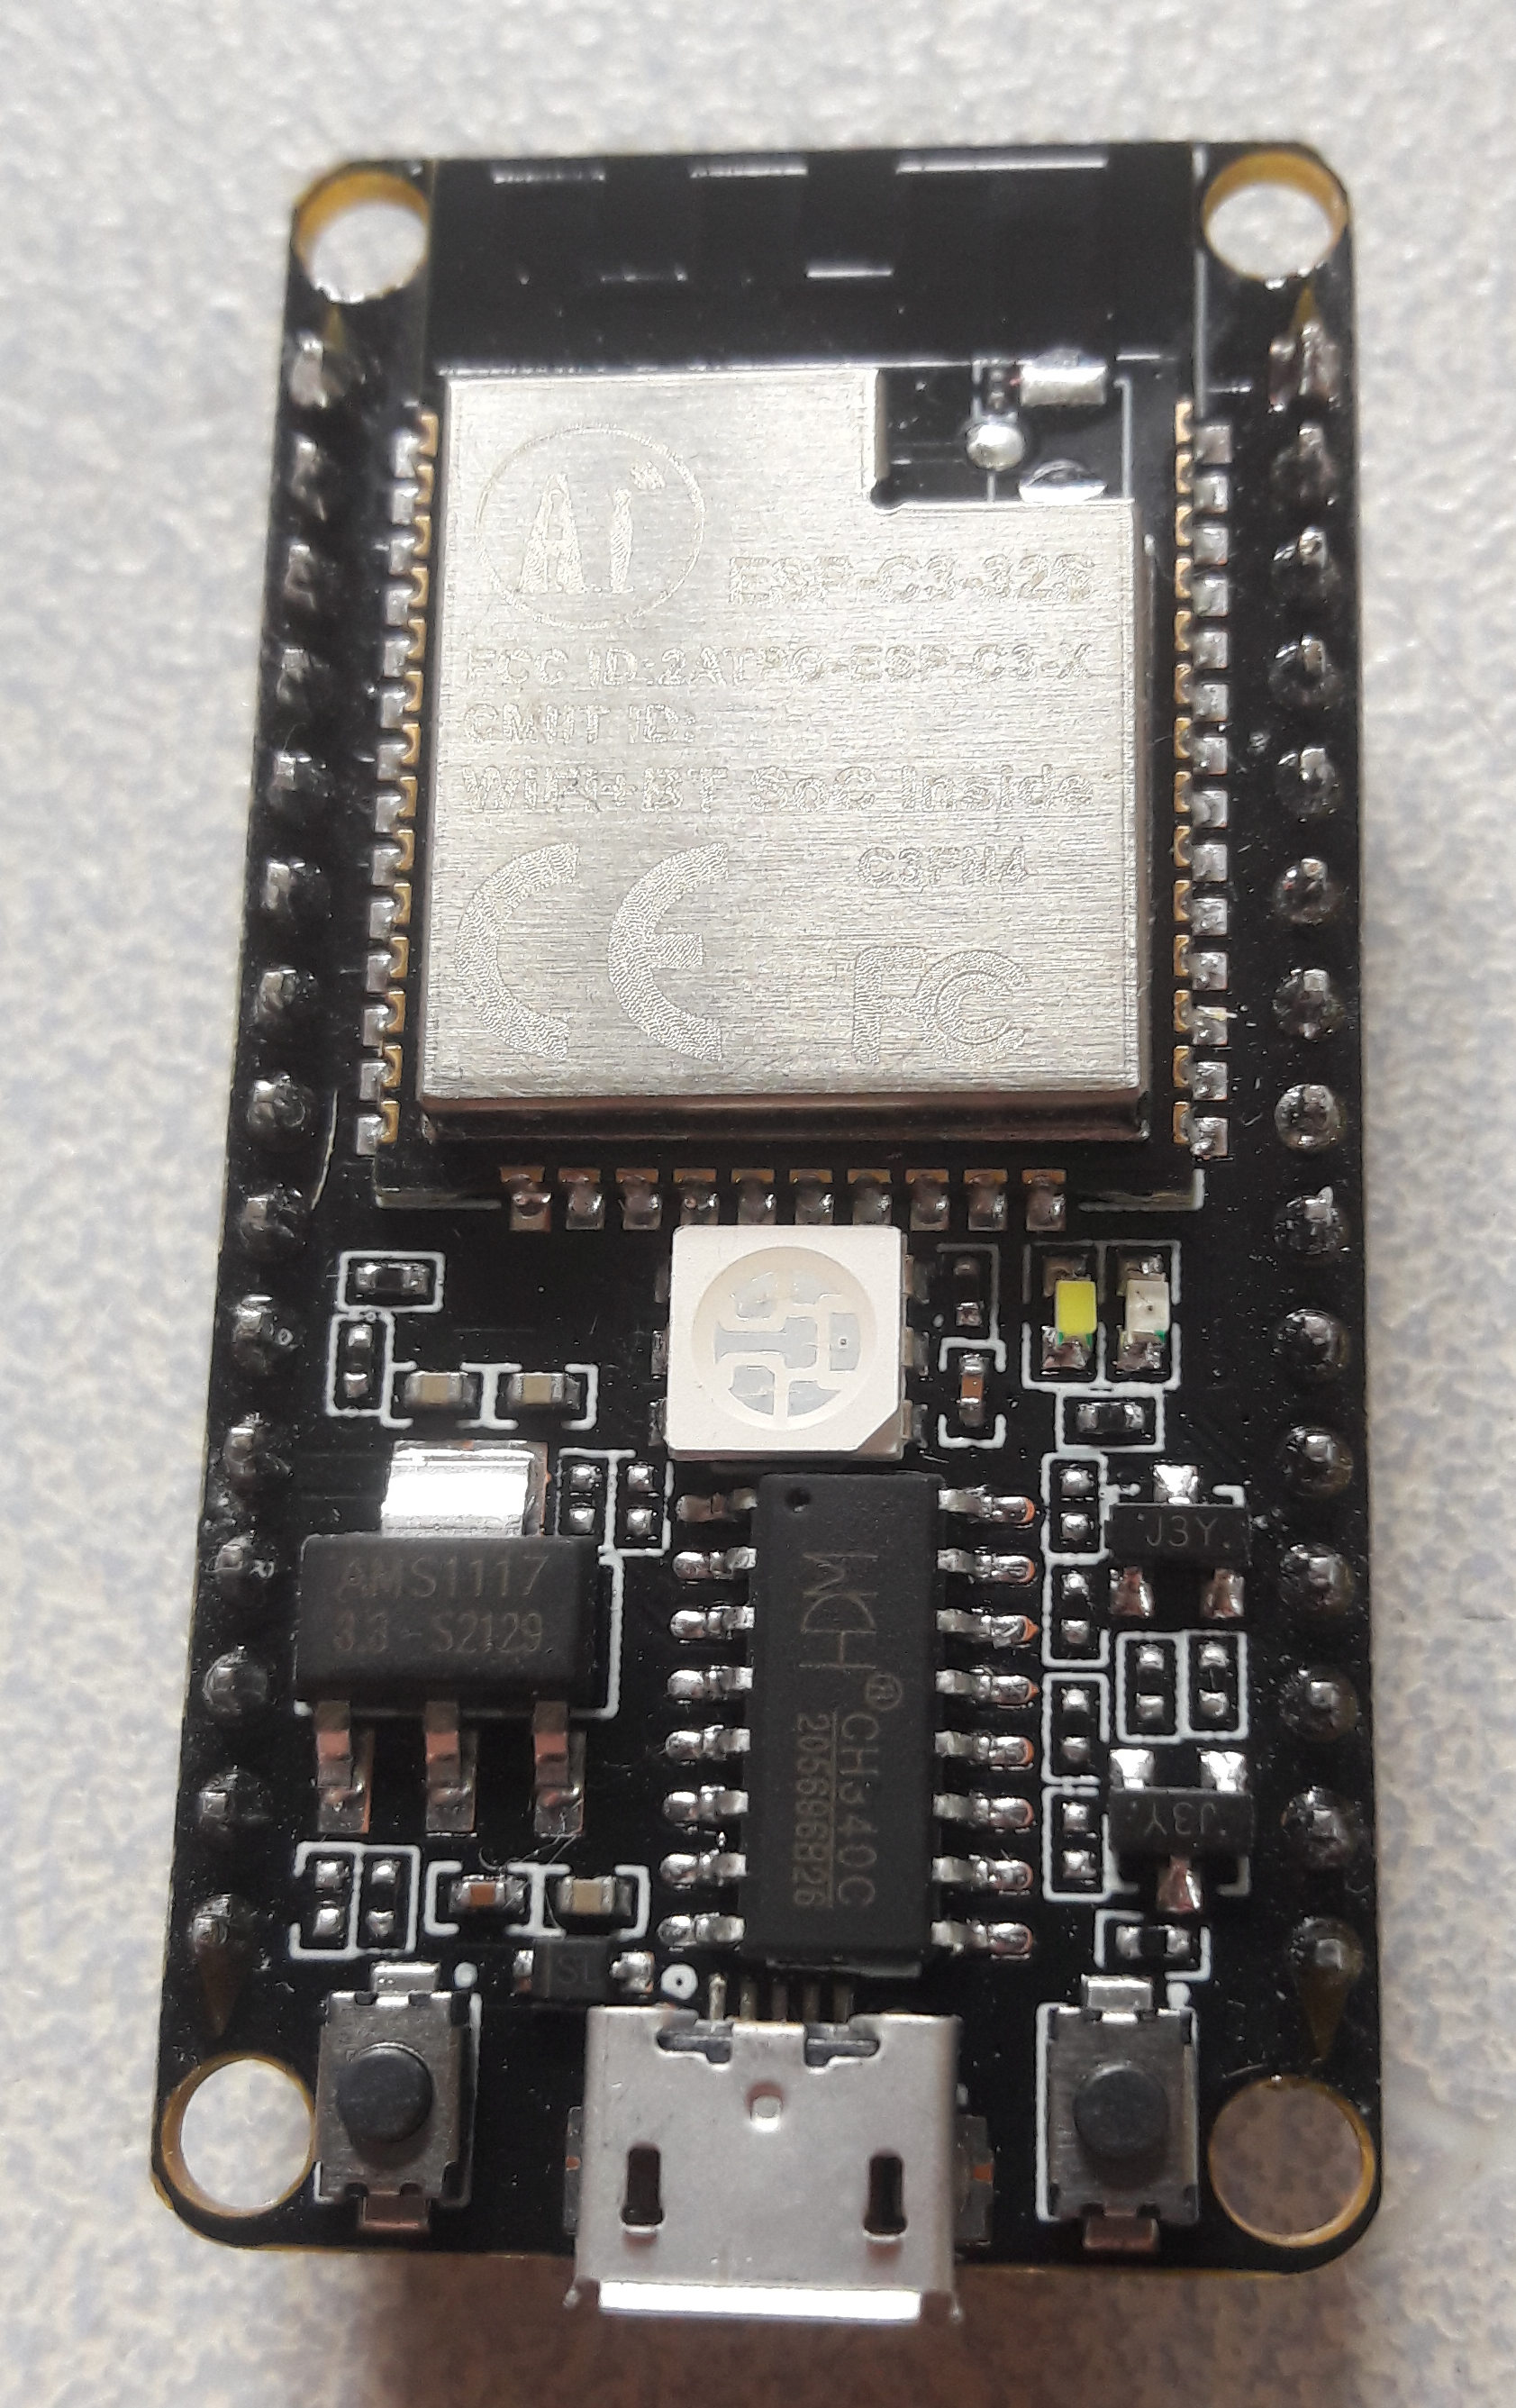
\includegraphics[width=0.3\paperwidth]{images/esp32-board}
        \caption{ESP32 en una tarjeta NodeMCU} \footnotesize
        Fuente: \textit{Wikipedia} $\mid$ ESP32. By Popolon - Own work, CC
        BY-SA 4.0, https://commons.wikimedia.org/w/index.php?curid=112634884.
    \end{figure}

    \subsection{Características}

    Las especificaciones completas de la tarjeta ESP32 se encuentran el la
    \href{https://www.espressif.com/sites/default/files/documentation/esp32_datasheet_en.pdf}{hoja de especificaciones}
    oficial, por lo que se enunciarán las características más destacables del producto a continuación \cite{espressif-systems-shanghai-co-ltd-2022B}:

    \begin{itemize}
        \item Wi-Fi 802.11 b/g/n, 802.11 n ($2.4GHz)$ hasta $150Mbps$,
        diversidad de antena, etc.

        \item Bluetooth v4.2 BR/EDR y LE, transmisor clase-1, clase-2,
        clase-3 sin amplificador de potencia externo, control de potencia, +9
        dBm de transmisión, etc.

        \item CPU Xtensa single-/dual-core $32 bit$ LX6.

        \item $448 KB$ de ROM.

        \item $520 KB$ de SRAM.

        \item $16 KB$ de SRAM en RTC.

        \item Oscilador inteno de $8 MHz$ con calibración.

        \item Oscilador RC interno con calibración.

        \item Un timer RTC, etc.

        \item $34$ GPIO programables.

        \item Boot seguro, encriptación mediante flash, algoritmos AES,
        SHA-2, RSA, ECC, RNG.

        \item Gran cantidad de aplicaciones como cámaras para streaming de
        video, robots para agricultura, reconocimiento de imágen, etc.
    \end{itemize}

    Las características son sin lugar a duda muy interesantes y completas. En
    tanto a las aplicaciones que se le pueden dar a este microcontrolador,
    son muchísimas.

    \bigbreak

    En el siguiente diagrama de bloques, se puede visualizar la arquitectura
    de esta tarjeta donde se destacan las características principales:

    \begin{figure}[H]
        \centering
        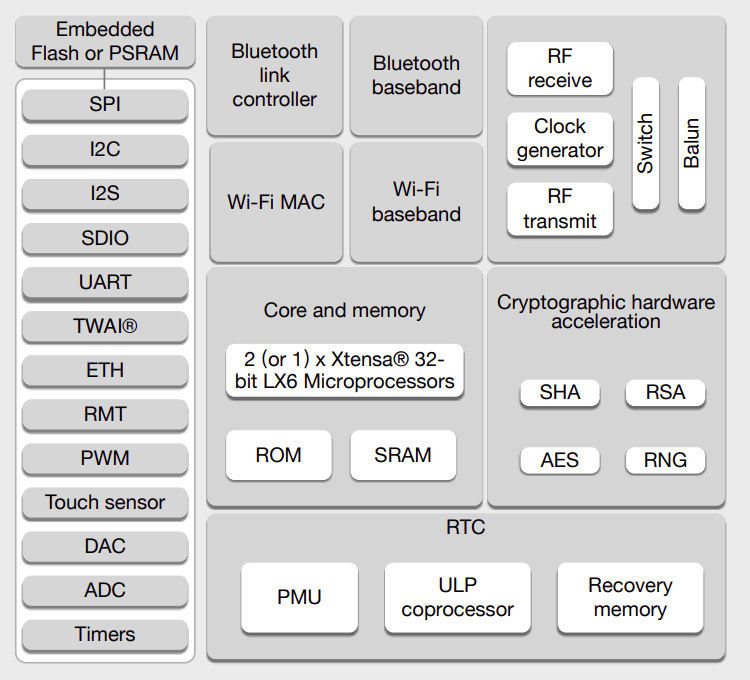
\includegraphics[width=0.3\paperwidth]{images/esp32-functional-block-diagram}
        \caption{ESP32 diagrama de bloque funcional} \footnotesize
        Fuente: \textit{ESPRESSIF} $\mid$ ESP32 Datasheet \cite{espressif-systems-shanghai-co-ltd-2022B} (bajo uso justo)
    \end{figure}

    O también, en esta otra la cual comparte mucha similitud:

    \begin{figure}[H]
        \centering
        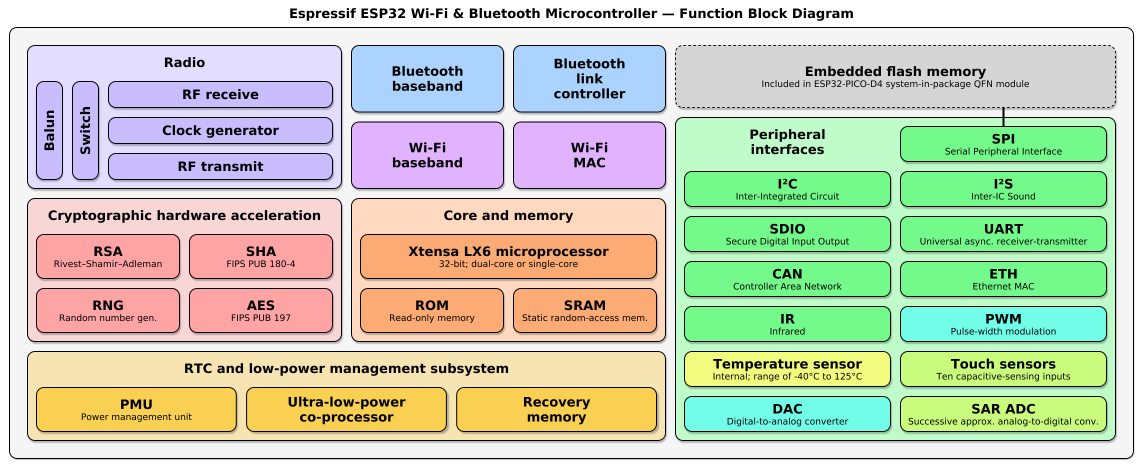
\includegraphics[width=0.3\paperwidth]{images/espressif-esp32-chip-function-block-diagram}
        \caption{ESP32 diagrama de bloque funcional (figura opcional)} \footnotesize
        Fuente: \textit{Wikipedia} $\mid$ ESP32. By Brian Krent (talk · contribs) - Own work, CC0, https://commons.wikimedia.org/w/index.php?curid=72304119.
\end{figure}

Para poder hacer uso del dispositivo, es importante saber su disposición de
pines, esto se obtiene de la siguiente documentación oficial:

\begin{figure}[H]
\centering
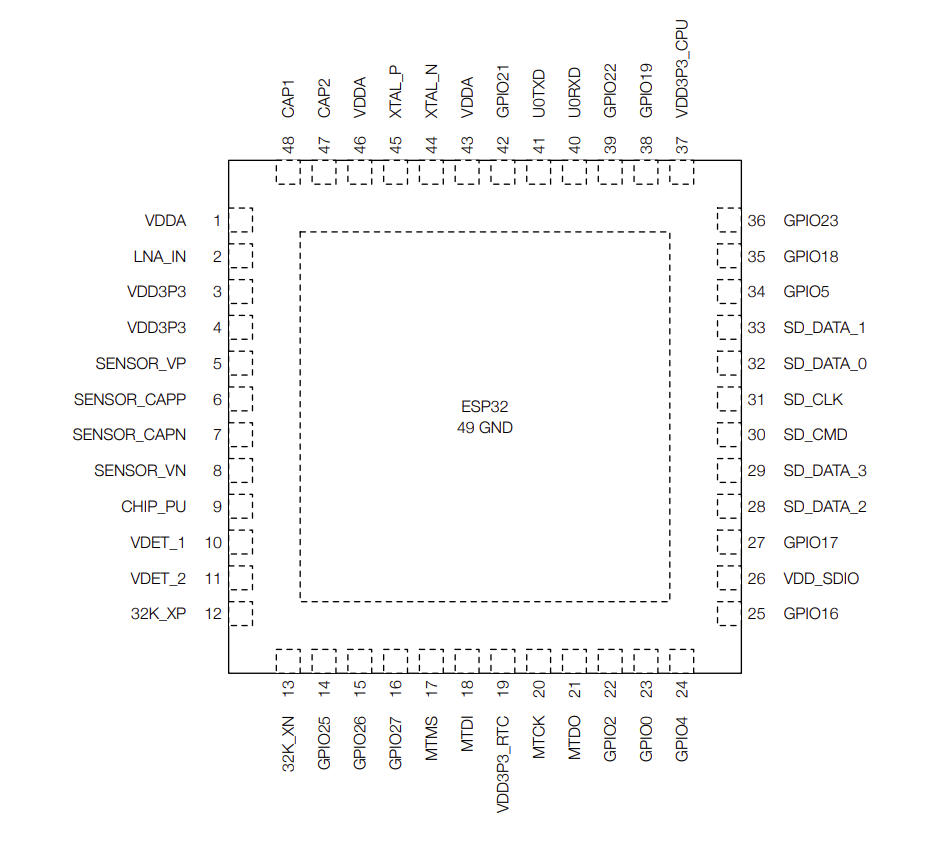
\includegraphics[width=0.3\paperwidth]{images/esp32-pin-layout.png}
\caption{ESP32 layout de pines (QFN 6*6, Vista desde arriba)} \footnotesize
Fuente: \textit{ESPRESSIF} $\mid$ ESP32 Datasheet \cite{espressif-systems-shanghai-co-ltd-2022B} (bajo uso justo)
\end{figure}

Por último, en \href{http://esp32.net}{http://esp32.net} se encuentran
también características y especificaciones, recursos de desarrollo para
muchos lenguajes de programación y plataformas, comunidades en línea sobre
este dispositivo en específico, lecturas y videos, plataformas de hardware,
información sobre proveedores que venden este dispositivo y otros accesorios
\cite{esp32net-esp32net-iot}.

\section{Desarrollo en Arduino IDE y C++}

En esta sección se tratará de abordar como poder crear un programa para la
tarjeta ESP32 mediante Arduino IDE y C++. En la siguiente sección, se verá
como es el proceso en MicoPython.

\bigbreak

Lo que se necesita hacer para establecer esta configuración es lo siguiente
\cite{pieters-2022}:

\begin{itemize}
\item Descargar e instalar Arduino IDE.

\item Ir a File - Preferences - Aditional Boards Manager URLs e ingresar la
dirección oficial para instalar la tarjeta ESP32 \url{https://dl.espressif
    .com/dl/package_esp32_index.json}.

\item Ir a Tools - Board - Boards manager.

\item Seleccionar la tarjeta ESP32 ya que se ha agregado al repositorio con
el paso anterior y proceder a instalarla.

\item Seleccionar la tarjeta que se tiene, de entre las tantas opciones.

\item Seleccionar el puerto USB ESP32 al conectar el módulo ESP.
\end{itemize}

Se usará la herramienta esptool para crear el firmware y flashearlo en la
tarjete ESP32.

\bigbreak

La tarjeta puede estar desacoplada, esto es, solamente el chip, o en una
tarjeta NodeMCU como se ilustró arriba. Utilizar Arduino IDE para flashear
esta tarjeta es más complicado ya que lleva varios pasos más. Claro está, es
Arduino IDE y no ESP32 IDE. Para esto, se tiene que resetear el
microcontrolador y empezar lo en modo flash usando GPIO-0 a Tierra. También
tener en cuenta sobre el programador que se va a emplear como se mencionó al
principio. Por último, para una forma visual y más profunda sobre este
proceso se puede consultar
\href{https://www.studiopieters.nl/esp32-program-a-esp32}{ESP32 - Program a ESP32 $\mid$ Studio Pieters}
\cite{pieters-2022}, así como también esta otra guía de mayor calidad
\href{https://www.electronicshub.org/esp32-arduino-ide}{How to Program ESP32 with Arduino IDE?} \cite{teja-2021}.

\subsection{Programa}

El siguiente programa puede ser usado para la ESP32. Es lo mismo que el C++
para Arduino, y se explica por si mismo.

\begin{lstlisting}[language=C, caption={Programa que hace parpadear el LED en
el pin 2}]
#define ledPin 2

void setup()
{
pinMode(ledPin, OUTPUT);
}

void loop()
{
digitalWrite(ledPin, HIGH);
delay(1000);

digitalWrite(ledPin, LOW);
delay(1000);
}
\end{lstlisting}

Para este programa, es probable que el LED (SMD) ya se encuentre en la
tarjeta, de lo contrario se tendrá que conectar un LED con su resistencia a
esta salida. La tarea de flashear la tarjeta con Arduino IDE es un poco
complicada, por lo que si no queda claro este aspecto, es muy recomendable
visitar los enlaces proveídos para entrar a más detalles.

\bigbreak

Para utilizar las entradas discretas, de igual forma, se utiliza \say{pinMode
(ledPin, INPUT);} para emplearla igual que cualquier programa Arduino.

\bigbreak

Se recomienda emplear MicroPython que se desarrolla en la siguiente sección
ya que funciona mejor para la tarjeta ESP32.

\section{Desarrollo con MicroPython}

Lo que nos proporciona la documentación de MicroPython para la tarjeta ESP32
es la siguiente información \cite{micropython-esp32}:

\begin{itemize}
\item Se obtienen los mejores beneficios al usar MicroPython en ESP32
(recordar que con Arduino IDE no fue tan bonito).

\item El software MicroPython soporta ESP32 y hay que tener en cuenta la
disposición de los pines, y si incluye un serial USB para tener el UART
disponible en el PC.

\item Verificar la alimentación de la tarjeta si no tiene USB.

\item Se debe descargar el \href{https://micropython.org/download/#esp32}{firmware}
de MicroPython para cargarlo en la tarjeta ESP32.

\item Para cargar el firmware se debe de primero, poner la tarjeta en modo
bootloader, y segundo, copiar el firmware. Esto depende de cada tarjeta por
lo cual se deberá consultar la documentación correspondiente para mayor detalle.

\item Para copiar el firmware, \href{https://github.com/espressif/esptool}{esptool}
es soportada por MicroPython y se debe tener instalada (pip install esptool).

\item Se borra el flash: esptool.py --port /dev/ttyUSB0 erase\_flash.

\item Y se despliega el firmware: esptool.py --chip esp32 --port /dev/ttyUSB0
write\_flash -z 0x1000 esp32-20180511-v1.9.4.bin.
\end{itemize}

\subsection{Programa}

Para la creación del programa se recomienda utilizar Thonny IDE. Entonces se
deberá de seleccionar en el IDE el intérprete y el puerto del dispositivo.
Ahí mismo en la pestaña de Intérprete, se selecciona en la parte de Firmware
para flashear el firmware que se descargó. El nombre del archivo debe ser
\say{main.py} ya que se carga \say{boot.py} de primero y luego \say{main.py}.

\bigbreak

\begin{lstlisting}[language=C, caption={Programa que hace parpadear un LED
hasta que se presiona el botón de salir en MicroPython. Fuente: Sparkfun
Electronics \cite{hymel}.}]
import machine
import sys
import utime

repl_button = machine.Pin(0, machine.Pin.IN, machine.Pin.PULL_UP)
led = machine.Pin(5, machine.Pin.OUT)

while True:
if repl_button.value() == 0:
print("Dropping to REPL")
sys.exit()

led.value(1)
utime.sleep_ms(500)
led.value(0)
utime.sleep_ms(500)
\end{lstlisting}

También se pude ver el otro ejemplo más detalladamente: Utilizar PWM para
controlar un LED de acuerdo a cuando se presione un botón pulsador.

\bigbreak

El código es el siguiente:

\begin{lstlisting}[language=C, caption={Programa que utiliza PWM en
MicroPython para ESP32. Fuente: Sparkfun Electronics \cite{hymel}.}]
import machine
import sys
import utime

repl_button = machine.Pin(0, machine.Pin.IN, machine.Pin.PULL_UP)
repl_led = machine.Pin(5, machine.Pin.OUT)
button = machine.Pin(14, machine.Pin.IN, machine.Pin.PULL_UP)
pwm_pin = machine.Pin(27, machine.Pin.OUT)
pwm = machine.PWM(pwm_pin)

while True:
if repl_button.value() == 0:
print("Dropping to REPL")
repl_led.value(1)
sys.exit()

for i in range(1024):
if button.value() == 0:
pwm.duty(i)
utime.sleep_ms(2)
else:
pwm.duty(0)
\end{lstlisting}

El diagrama es el siguiente:

\begin{figure}[H]
\centering
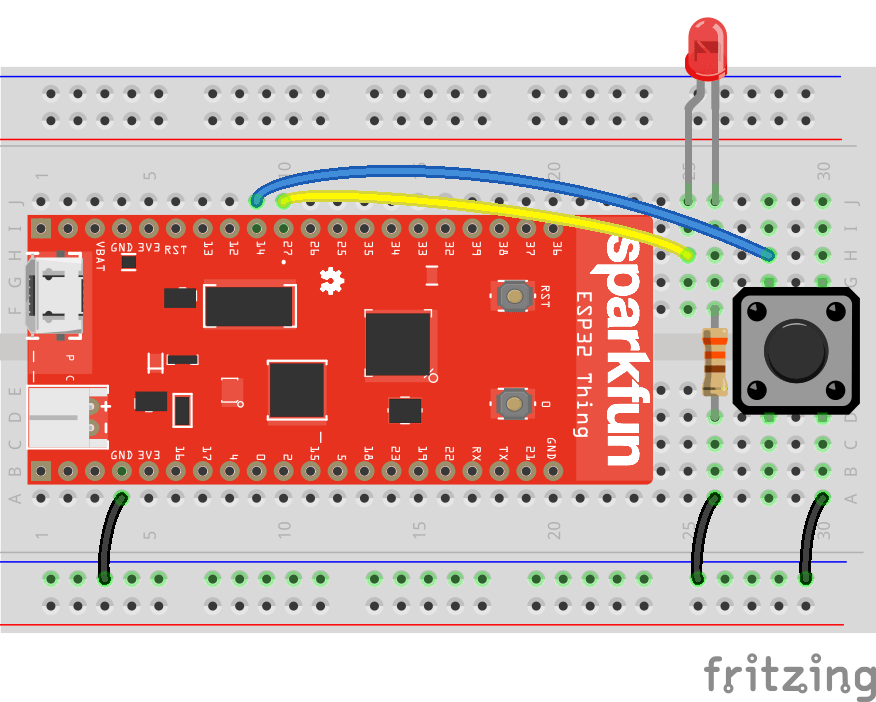
\includegraphics[width=0.3\paperwidth]{images/esp32-micropython-pwm-circuit}
\caption{Circuito para programa PWM con MicroPython} \footnotesize
Fuente: \textit{Sparkfun} $\mid$ MicroPython Programming Tutorial: Getting
Started with the ESP32 Thing \cite{hymel} (under the CC BY-SA 4.0 license)
\end{figure}

Y se ve algo así:

\begin{figure}[H]
\centering
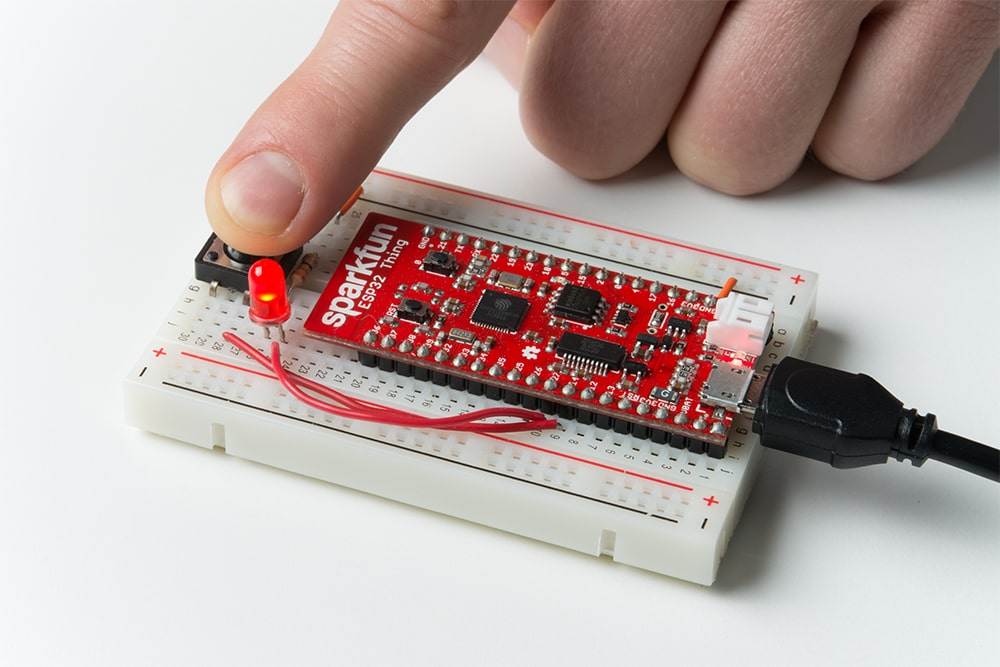
\includegraphics[width=0.3\paperwidth]{images/esp32-micropython-pwm-photo}
\caption{Resultado para programa PWM con MicroPython} \footnotesize
Fuente: \textit{Sparkfun} $\mid$ MicroPython Programming Tutorial: Getting
Started with the ESP32 Thing \cite{hymel} (under the CC BY-SA 4.0 license)
\end{figure}

\section{Conclusión}\label{sec:conclusion}

Se explicó brevemente las características y pasos principales de la tarjeta
microcontrolador ESP32 para poder emplear ya sea Arduino IDE o MicroPython
para el desarrollo de aplicaciones para ESP32. Se vio el uso de entradas y
salidas digitales tanto en C++ Arduino y en MicroPython, adicionando un
proyecto PWM para MicroPython. Por último, se recomendó emplear MicroPython
para un mejor uso de la tarjeta ESP32.

\printbibliography

\end{document}
